% Created 2015-02-18 Wed 14:32
\documentclass[presentation]{beamer}
\usepackage[utf8]{inputenc}
\usepackage[T1]{fontenc}
\usepackage{fixltx2e}
\usepackage{graphicx}
\usepackage{longtable}
\usepackage{float}
\usepackage{wrapfig}
\usepackage{rotating}
\usepackage[normalem]{ulem}
\usepackage{amsmath}
\usepackage{textcomp}
\usepackage{marvosym}
\usepackage{wasysym}
\usepackage{amssymb}
\usepackage{hyperref}
\tolerance=1000
\definecolor{myPrimary}{RGB}{45,217,0}
\definecolor{mySecondary}{RGB}{0,162,87}
\definecolor{myTertiary}{RGB}{255,67,0}
\setbeamercolor{structure}{fg=myPrimary,bg=mySecondary}
\setbeamercolor{palette primary}{fg=myPrimary}
\setbeamercolor{palette secondary}{fg=mySecondary}
\setbeamercolor{palette tertiary}{fg=myTertiary}
\usepackage{droid}
\usetheme{PaloAlto}
\author{Hermann Pauly}
\date{}
\title{Visualisation for \emph{segemehl} output}
\hypersetup{
  pdfkeywords={},
  pdfsubject={},
  pdfcreator={Emacs 24.4.1 (Org mode 8.2.10)}}
\begin{document}

\maketitle

\section*{Introduction}
\label{sec-1}

\begin{itemize}
\item \emph{segemehl}: alignment tool for NGS
\item can map strand switching and circular events
\item no software to plot output yet
\end{itemize}

\subsection*{Goal}
\label{sec-1-1}

\begin{itemize}
\item tool to create plots from \emph{segemehl} mappings
\item allow search for "unusual" splice events
\item user-defined selection and filtering of plots
\end{itemize}

\section*{My approach}
\label{sec-2}

\begin{itemize}
\item graph theory
\item on-screen and file output
\item C++, Qt4, \emph{.eps}
\end{itemize}

\subsection*{Read as graph}
\label{sec-2-1}

\begin{itemize}
\item test data
\begin{itemize}
\item simulated chromosomes
\item manually created RNA-reads
\item re-mapped with segemehl
\end{itemize}
\item real data
\begin{itemize}
\item RNA sequences of human skin cells
\item already mapped by \emph{segemehl}
\end{itemize}
\end{itemize}

\subsection*{Datastructure: reassembly}
\label{sec-2-2}

\begin{itemize}
\item exons as nodes
\item splicings as edges
\item chromosomes: maps of links to nodes
\end{itemize}

\subsection*{Datastructure: plotting}
\label{sec-2-3}

\begin{itemize}
\item chromosomes (name, length, exon pos)
\item exons for plots (id, length, position)
\item connection information
\end{itemize}

\section*{Results}
\label{sec-3}

\subsection*{Multisplit plot}
\label{sec-3-1}

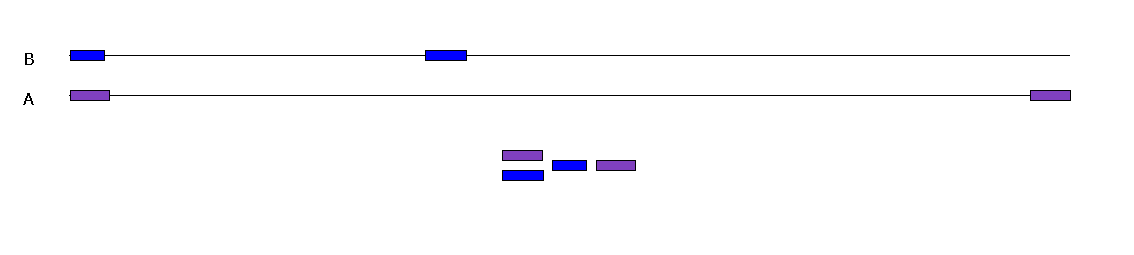
\includegraphics[width=.9\linewidth]{./cb2/snapshot1.png}
(test data, 3' -> 5')

\subsection*{Profiling}
\label{sec-3-2}

\begin{verbatim}
index % time    self  children    called     name
                                                 <spontaneous>
[1]     97.6    0.00    3.27                 main [1]
[2]     96.9    0.00    3.24       1         Genome::read(std::string&) [2]
[3]     96.9    0.01    3.23       1         Genome::read(std::basic_ifs...
[4]     84.2    0.08    2.74  199914         Genome::parseDataLine(std::...
-----------------------------------------------
                0.00    0.00     253/200167      Genome::parseHeaderLine...
                0.05    1.66  199914/200167      Genome::parseDataLine(s...
[5]     51.1    0.05    1.66  200167         strsplit(std::string, std::...
                0.06    1.04 3579101/3579185     std::vector<std::string...
                0.00    0.24  200167/200167      std::vector<std::string...
                0.03    0.09  200167/200167      std::unique_ptr<std::ve...
                0.04    0.07 3779268/3779268     bool std::operator!=<ch...
                0.03    0.04 3579101/3579101     std::unique_ptr<std::ve...
                0.00    0.03  200167/200167      std::unique_ptr<std::ve...
                0.00    0.00  200167/200167      std::unique_ptr<std::ve...
                0.00    0.00  200167/200168      std::vector<std::string...
\end{verbatim}

\section*{Problems and outlook}
\label{sec-4}

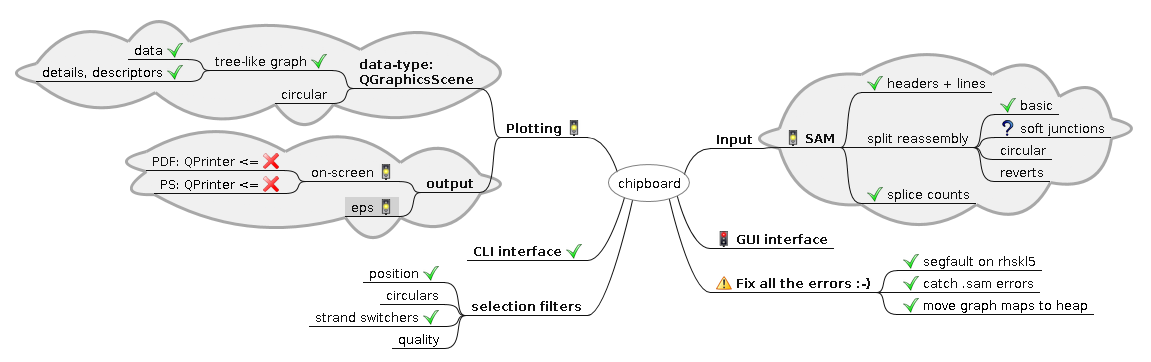
\includegraphics[width=.9\linewidth]{./cb2/roadmap.png}

\subsection*{Problems}
\label{sec-4-1}

\begin{itemize}
\item \emph{segemehl} doesn't honour \emph{.sam} standard
\item memory: graph of 40+ GiB input files
\item data not ordered
\item Qt4 file printing surprisingly bad
\end{itemize}

\subsection*{To do / planned}
\label{sec-4-2}

\begin{itemize}
\item visuals
\begin{itemize}
\item include strandiness information
\item shortened chromosome displays
\item more information
\end{itemize}
\item function
\begin{itemize}
\item more filtering
\item circular elements
\item graphical interface
\item more input formats
\item include genomic annotation
\end{itemize}
\end{itemize}

\section*{}
\label{sec-5}
\alert{Thank you}

\section*{Sources}
\label{sec-6}

\section*{strsplit()}
\label{sec-7}

\begin{verbatim}
vector<string> strsplit ( string& input, string& delim, bool keepEmpty ) {
  string token, theStr(input);
  int L = delim.length();
  vector<string> result(new vector<string>());

  while (token != theStr) {
    auto end = theStr.find_first_of(delim);
    token = theStr.substr(0, end);
    theStr = theStr.substr(end + L);
    if (keepEmpty || token.length() > 0) {
      result.push_back(token);
    }
  }
  return result;
}
\end{verbatim}
% Emacs 24.4.1 (Org mode 8.2.10)
\end{document}